\documentclass{IEEEcsmag}

\usepackage[colorlinks,urlcolor=blue,linkcolor=blue,citecolor=blue]{hyperref}

\usepackage{tabularx}
\usepackage{upmath}
\usepackage{amssymb}
\usepackage{amsmath}
\usepackage{array}
\usepackage{arydshln}

\newcolumntype{P}[1]{>{\centering\arraybackslash}p{#1}}

\jvol{XX}
\jnum{XX}
\paper{8}
\jmonth{May/June}
\jname{Computing in Science and Engineering}
\pubyear{2021}
\newtheorem{theorem}{Theorem}
\newtheorem{lemma}{Lemma}

\setcounter{secnumdepth}{0}

\begin{document}

\sptitle{Department: Head}
\editor{Editor: Name, xxxx@email}

\title{PyExaFMM, an exercise in designing high-performance software with Python and Numba}

\author{S. Kailasa}
\affil{Department of Mathematics, University College London}

\author{T. Wang}
\affil{Department of Mechanical and Aerospace Engineering, The George Washington University}

\author{\text{L}. A. Barba}
\affil{Department of Mechanical and Aerospace Engineering, The George Washington University}

\author{T. Betcke}
\affil{Department of Mathematics, University College London}

\markboth{Department Head}{Paper title}

\begin{abstract}
    Python's dramatic rise in popularity for computational science, and its use as first language for many scientists and engineers makes it important to optimize. 
\end{abstract}

\maketitle
\chapterinitial{CPython} is the most popular implementation of the dynamically typed and interpreted, Python programming language. CPython was designed with safety and productivity in mind, rather than high-performance computing [HPC]. Pythons's dynamic typing forces objects to be passed through an interpreter loop at runtime, and applications are restricted to a single thread via a `global interpreter lock' [GIL] to ensure thread safety. However, Python's popularity has lead to the development of numerous open-source tools for HPC with CPython, that allow users to bypass the interpreter, develop multithreaded applications, and even deploy source code written in Python to GPUs.

PyExaFMM\footnote{https://www.github.com/exafmm/pyexafmm} is a solver for the three-dimensional particle fast multipole method [FMM] \cite{Greengard1987}, designed to be run on single-node multicore architectures. It was designed to test the efficacy of Numba, a `just-in-time' [JIT] compiler, for developing HPC applications in CPython. Building on the success of the ExaFMM project's comparable C++ implementation \cite{Wang2021}, we sought to test whether the productivity benefits of working in Python could be retained while achieving performance comparable to compiled languages.  The FMM consists of a recursive loop through a hierarchical data structure. Representing computations and data efficiently while retaining performance is challenging, therefore it offers a good benchmark for studying the efficacy of Python and Numba for developing efficient software for complex algorithms.

\section{NUMBA}

Numba bypasses the interpreter for operations involving loops over Numpy arrays and numeric scalars, translating Python source code into efficient platform-dependent machine code using the LLVM infrastructure. LLVM applies hardware dependent optimizations such as single-instruction multiple data [SIMD] vectorization over loops, to the intermediate bytecode representation [IR] produced by Numba. Bypassing the interpreter in this way can make Numba compiled functions competitive with compiled languages. However, we note that Numba is not able to map operations specified in Python to efficient machine instructions if they contain functionality outside of its numeric remit. Furthermore, Numba still requires interaction with the Python interpreter to pass data to Numba compiled functions, as well as to interact with non-optimized parts of the codebase involved in data-organization or calls to incompatible libraries. Therefore, developers have to organize their code to restrict interaction with the Python interpreter, and ensure that their methods can be optimized by Numba, to see a performance benefit from using it.

Functions are marked for JIT compilation with a decorator, and `polymorphic dispatching' picks up the type signature from the arguments used at runtime - running compilation for a function with this signature if it does not already exist in cache. The compiled function is called from a Python wrapper which forms the interface between the Python runtime and a Numba compiled function. Therefore Numba fits easily into existing Python projects. Numba has been extended with efficient implementations of many of the array manipulation and linear algebra operations offered by Numpy, as well as multithreading functionality via iterations over a parallel range iterator, reminiscent of OpenMP's parallel for loops. Furthermore, Numba supports the writing of Python kernels for AMD and NVidia GPUS, and is fully integrated with the CuPy library.

Therefore, Numba provides a `framework' for developing heterogenous, cross-platform, applications using only Python source code. This framework impacts the design of software as performance is dictated by the interaction between the Python interpreter and Numba optimized functions. Developers have to be careful to design Numba functions that are vectorizable, and multithreaded functions that are cache-optimal. Methods have to limit the usage of Python objects, and instead be designed around Numpy arrays. In this paper we begin by briefly summarizing the kernel independent FMM [KIFMM] algorithm used by PyExaFMM, before proceeding to describe the mathematical optimizations, and software design strategies we used for achieving performance with Numba. We discuss how we parallelize FMM operations to maximize cache-reuse, our approach to designing functions for Numba compilation, as well as how we architected PyExaFMM to minimize interactions between Numba compiled functions and the Python interpreter. We conclude with benchmarks comparing the memory usage, runtimes and accuracy of the software with respect to the comparable state-of-the-art C++ implementation from the ExaFMM project, ExaFMM-T \cite{Wang2021}.

\section{THE FAST MULTIPOLE METHOD}

The particle FMM is an algorithm for approximating the $N$-body problem, in which one aims to calculate the pairwise interactions between $N$ particles. Consider a domain $ D \subset \mathbb{R}^3$, containing a set of `source' particles at positions $x_i$, and their interaction with a `target' particle at position $y_j$ where $i \in [1,...,N]$, and $x_i, y_j \in \mathbb{R}^3$. The pairwise interaction of the target with all sources can be written as,

\begin{flalign}
	\label{eq:n_body_problem}
	\phi_j = \sum_{i=1}^{N}K(x_i, y_j)q_i
\end{flalign}

where $K(., .)$ is called the `kernel' or Green's function, and the interactions are weighted by $q_i$. This calculation appears in numerous contexts across science and engineering. For example, if we interpret $q_i$ as a charge, and take the Green's function to be,

\begin{flalign}
	K(x, y) = \frac{1}{4\pi|x-y|}
	\label{eq:laplace_kernel}
\end{flalign}

called the `Laplace kernel', we recognize (\ref{eq:n_body_problem}) as the calculation of the electrostatic potential $\phi_j$ at $y_j$ due to source particles at positions $x_i$ with charges $q_i$. Without loss of generality we can consider the sources and targets to correspond to the same set of particles, and take this as our benchmark problem. A naive calculation of (\ref{eq:n_body_problem}) at $N$ target positions results in an algorithm of $\mathcal{O}(N^2)$ runtime. The FMM is able to approximate this in $\mathcal{O}(N)$, with well-defined error bounds. It works by partitioning $D$ using a hierarchical tree. Level $0$ of the tree corresponds to a cubic box containing all source and target particles, it is then recursively partitioned into $8^l$ boxes where $l$ is a given level. The maximum level $l$, or \textit{leaf level}, of partitioning in a subset of $D$ is set by a user defined constant for the maximum number of particles allowed in a leaf box. Refinement proceeds uniformly across the domain until this condition is satisfied. Optionally, the domain can be refined in a \textit{non-uniform} manner such that the leaf level consists of boxes of different sizes, reflecting non-uniform particle distributions. The level of non-uniformity in the final tree can be restricted by a \textit{balance condition}, which dictates the maximum difference in size between two neighboring boxes. Figure (\ref{fig:algorithm}b) illustrates the relationship between a given leaf box $T$ and surrounding boxes, termed \textit{interaction lists}, for a non-uniform tree in $\mathbb{R}^2$. The $U$ list consists boxes adjacent to $T$ - i.e. sharing an edge or vertex (or face in $\mathbb{R}^3$), known as its \textit{neighbors}. Neighbors at the same level of discretization are known as \textit{colleagues}.  The $V$ list consists of child boxes of the colleagues of $T$'s parent box, which are not-adjacent to $T$. The $W$ list consists of descendent boxes of $T$'s colleagues, which are not-adjacent to $T$, and the $X$ list consists of boxes for which $T$ is in the $W$ list. The $X$ and $W$ lists only occur in non-uniform trees, and are only formed for leaf boxes.

The FMM consists of six operators: P2M, M2M, M2L, L2L, L2P and P2P, where a given operator is read as `X to Y'. `P' stands for particle(s), `M' for multipole expansion and `L' for local expansion. The operators are translations between expansion representations. A multipole expansion represents the aggregation of charge located within a given box in the tree, in the FMM we choose to set the expansion center to coincide with the box center. It can be truncated to an `expansion order', $p$, for tunable accuracy. A multipole expansion can be translated into a local expansion centered on another box, inside of which it is valid. This is the M2L operator. Similarly the expansion centers of local or multipole expansions can be shifted, which are the L2L and M2M operators respectively. The P2M operator is the act of forming a multipole expansion for a set of particles within a box. L2P and P2P refer to direct evaluations using (\ref{eq:n_body_problem}) between local expansion coefficients, or source particles, with a set of target particles, respectively.

Figure (\ref{fig:algorithm}) illustrates the FMM for a problem in $\mathbb{R}^2$. Figure (\ref{fig:algorithm}a) shows the recursive partition, and the \textit{upward pass}. The tree is traversed bottom-up, multipole expansions are found leaf boxes (P2M), their centers are shifted to the center of their parent box (M2M) and expansion coefficients summed in order to find the parent multipole expansion. Figure (\ref{fig:algorithm}c) and Figure (\ref{fig:algorithm}d) show the \textit{downward pass}. The tree is traversed top-down, starting at level $2$. M2L transfers for source boxes in a target box's $V$ list are performed and accumulated as a local expansion, followed by L2L transfers, where its expansion coefficients are added its children's. Local expansions compress the far field component of potential for targets within a given leaf box, and are evaluated directly at its target particles (L2P). The far field is defined by a box and its ancestors' $V$ lists. The near field is defined by its $U$, $W$ and $X$ lists, and is evaluated directly for boxes at the leaf level (P2P). The P2P step can be made more efficient for non-uniform trees by using the $X$ and $W$ lists. Consider a leaf box $T$, we can use the multipole expansion of boxes in its $W$ list to evaluate their contribution towards potential for target particles in $T$ (M2P). For boxes in $T$'s $X$ list, we can evaluate the source charges directly at the points supporting the local expansion (S2L), before performing L2P, where `S' stands for source particles.

The far field contribution to potential is compressed in the local expansion for a given box, and is found by performing M2L transfers over its $V$ list, the size of which is bounded by a constant. Therefore we see the complexity of the FMM to be dictated by the number of nodes in the tree, which due to the maximum particle per node constraint will be restricted to $\mathcal{O}(N)$.

In the KIFMM \cite{Ying2004}, we use evaluations of the kernel function, rather than series expansions, to find multipole and local expansions and to translate between them. Consider the P2M operator for a given box illustrated in figure (\ref{fig:operators}a). The multipole expansion is described by equivalent charges placed at $n$ quadrature points evenly spaced on an \textit{equivalent surface} enclosing the box. Where $n$ is related to the expansion order $p$ by,

\begin{flalign}
	n = 6(p-1)^2+2
	\label{eq:order}
\end{flalign}

The sum (\ref{eq:n_body_problem}), for these equivalent charges is matched to the \textit{check potential} $\phi^c$ calculated from the charges in the box directly at quadrature points on a \textit{check surface} that encloses the equivalent surface and the box. Each component of $\phi^c$, corresponding to a point on the check surface $y_j$, is calculated as,

\begin{flalign}
	\phi_{j}^c = \sum_{i=1}^{N_{box}} K(x_i, y_j) q_i
\end{flalign}

where there $N_{box}$ particles in the box, with charges $q_i$ and at positions $x_i$. We find the equivalent charges $q^e_i$ corresponding to points $x_i$ on the equivalent surface with,

\begin{flalign}
	\sum_{i=1}^{N_{e}} K(x_i, y_j)q^e_i = \phi^c
\end{flalign}

Where $N_e$ is the number of quadrature points on the equivalent surface. In matrix form,

\begin{flalign}
	K q_{e} = \phi^c \\
	q_e = K^{-1} \phi^c
	\label{eq:p2m}
\end{flalign}

The matrix on the right hand side of (\ref{eq:p2m}) is taken to be the P2M operator. This logic is repeated to form the other KIFMM operators, the required check and equivalent surfaces and matchings are illustrated in figure (\ref{fig:operators}). We note that for the L2L and M2L operators, the equivalent surface around the target box encloses the check surface, which itself encloses the target box. This is reflective of the region of validity of local expansions. The check potentials are then formed with the child/parent equivalent charges for the M2M and L2L operators respectively, and with the equivalent charges of boxes in the $V$ list of a given box, for its corresponding M2L operator. The L2P, M2P, S2L and P2P operators are evaluated directly using (\ref{eq:n_body_problem}). We note that large values of $p$ lead to poor conditioning in the inversion of the matrix $K$, and in practice we solve this by taking the \textit{backward-stable pseudo-inverse} of $K$, introduced by Malhotra et. al \cite{Malhotra2015}.

% Larger figure
\begin{figure*}
	\centerline{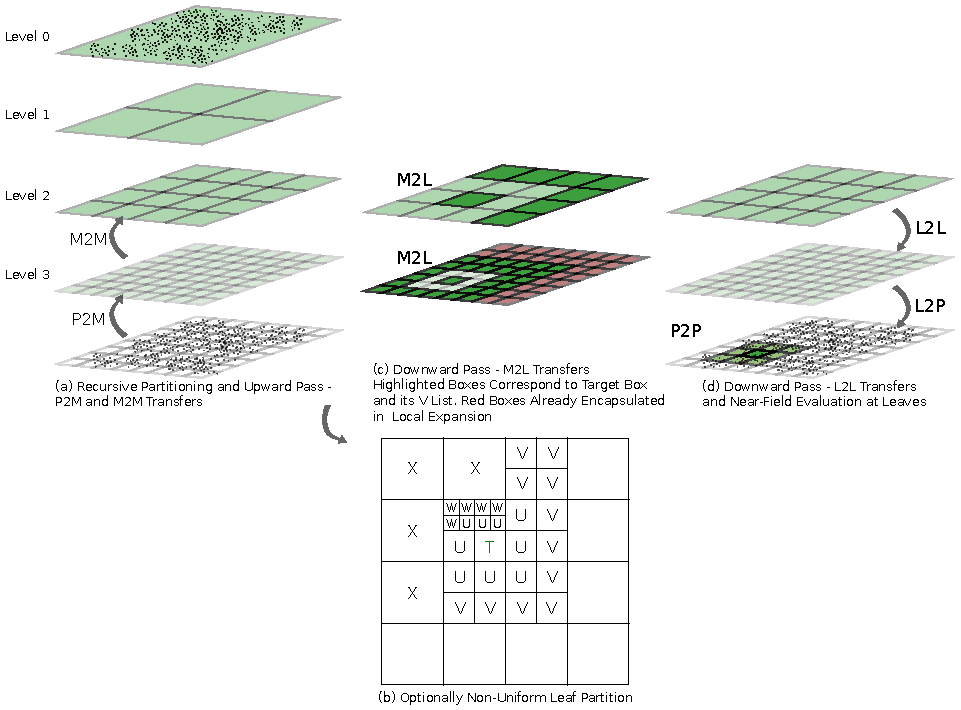
\includegraphics {figures/tree.pdf}}
	\caption{FMM algorithm and operator actions, including tree construction, illustrated for problem in $\mathbb{R}^2$.}
	\label{fig:algorithm}
\end{figure*}

\begin{figure*}
	\centerline{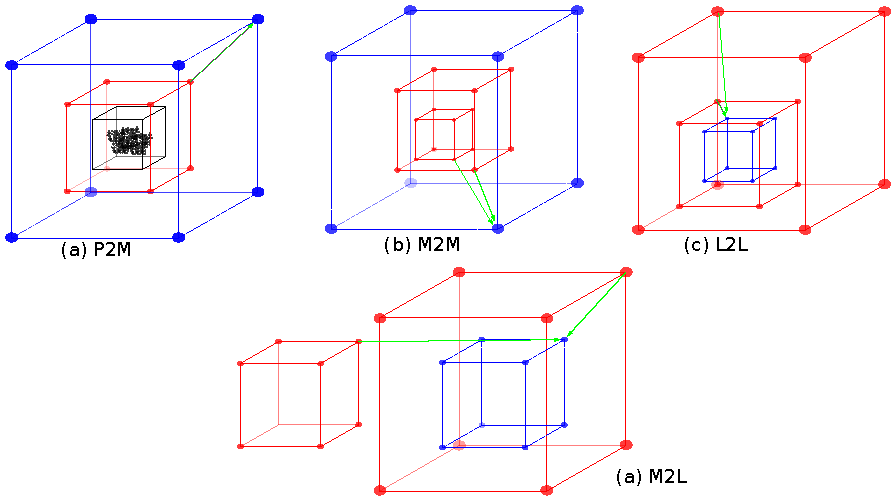
\includegraphics {figures/operators.pdf}}
	\caption{KIFMM operator calculations for order $p=2$ expansions. Equivalent charges placed at quadrature points on the (red) equivalent surfaces, are matched at quadrature points on the (blue) check surfaces. Charges are plotted in black, and green arrows are used to indicate matchings.}
	\label{fig:operators}
\end{figure*}


\section{TECHNIQUES FOR ACHIEVING PERFORMANCE}

\subsection{Compressing the M2L Operator with SVD}

The maximum size of a $V$ list in three dimensions [3D] is 189. Therefore, naively forming M2L matrices, and performing inversions for each box during the downward pass is expensive. Instead, we label each unique $V$ list interaction at a given tree level with a \textit{transfer vector} \cite{Fong2009}. Note that there are at most $7^3-3^3=316$ transfer vectors at a given level. As usual we seek the equivalent charge around a target box due to a source box in its $V$ list, by matching the kernel evaluations at a check surface enclosing the target box and its equivalent surface,

\begin{flalign}
	K^{se2tc} q^s_e = K^{te2tc} q^t_e
\end{flalign}

where $K^{se2tc}$ is the matrix with elements calculated using (\ref{eq:laplace_kernel}), between the source box's equivalent surface, and a target box's check surface, $K^{te2tc}$ is calculated using the target box's equivalent and check surfaces, $q^s_e$ is the known equivalent charge at the source box (multipole expansion), and $q^t_e$ is the unknown equivalent charge at the target box (local expansion). We form the M2L matrix by inverting $K^{te2tc}$,

\begin{flalign}
	q^t_e = \underbrace{(K^{te2tc})^{-1} K^{se2tc}}_{M2L} q^s_e
\end{flalign}

We can form an M2L matrix at level $l$, for source boxes corresponding to all unique transfer vectors, and concatenate them,

\begin{flalign}
	M2L_{l} = \begin{pmatrix}
M2L_1 & M2L_2 & ... &  M2L_{316}
\label{eq:concatenated_m2l}
\end{pmatrix}
\end{flalign}

where $M2L_l \in \mathbb{R}^{N_c \times 316N_e}$, and $N_c$ and $N_e$, are the number of quadrature points on the check and equivalent surfaces, respectively. When we encounter an M2L interaction during the downward pass, we simply compute the corresponding transfer vector and look up the sub-matrix of (\ref{eq:concatenated_m2l}) that corresponds to its M2L matrix. Matrix (\ref{eq:concatenated_m2l}) can be pre-computed and cached. PyExaFMM further reduces the application and storage costs of (\ref{eq:concatenated_m2l}) at a given level by applying \textit{SVD compression}. Consider taking the SVD of $M2L_l$

\begin{flalign}
	M2L_l = \sum_{j=1}^r \sigma_ju_jv_j^T
	\label{eq:compressed_m2l}
\end{flalign}

where the row-rank $r=\text{rank}(M2L_l) = N_c$, $u_j$ and $v_j$ are the left and right singular vectors respectively, and the singular values $\sigma_j$ are arranged in weakly decreasing order. We can cutoff this sum at a \textit{compression rank} $k \leq N_c$ to approximate $M2L_l$. PyExaFMM implements the \textit{randomized SVD} of Halko et. al \cite{Halko2011}. The algorithm can be decomposed into a series of BLAS level 2 and 3 operations, making it fast to compute for large matrices.


\subsection{Efficiently Representing Trees and Expansions}

Particle coordinates are discretized into tree boxes via a \textit{Morton encoding} \cite{Sundar2007}. The relative position of a box at a given level $l$, can be described in terms of integer displacements along each coordinate axis in the range $[0, 2^l)$, with respect to a corner of the root box chosen to be the `origin'. The bits of these \textit{indices} are interleaved as,

\begin{flalign}
	x_1 y_1 z_1 x_2 y_2 z_2...x_n y_n z_n | l
\end{flalign}

where $x_i$, $y_i$ and $z_i$ are the $i^{th}$ bit of the respective index, and the level is appended to the end. This is known as a \textit{Morton key}. We can map between physical particle coordinates and Morton keys at a given level by scaling the physical coordinates with respect to the boxes at this level, and finding their relative displacement from the origin. Morton keys are stored as signed 64 bit integers\footnote{Python doesn't support all bitwise shifts on unsigned integers.}, with $15$ bits for the level $l$, and $16$ bits for the index along a given axes. They allow for simple calculation of tree relationships. For example, the parent of a given box - by removing the last three bits and subtracting one from the level; its children - by appending the appropriate combinations onto the final three bits and adding one to the level; or its neighbours - which are defined by algebraic displacements of the index bits. These operations are efficiently represented by Numba as they only use arithmetic operations and bit shifts.

PyExaFMM represents trees linearly as an array of Morton keys, and enforces a \textit{2:1 balance}, such that neighboring boxes differ by at most one level. Containers for the multipole and local expansions at each box, as well as for calculated potential and potential gradients at each target, are stored in linear arrays. They are linked to the tree via lookup tables, stored as Numba compatible dictionaries, where the Morton key can be used to look up the associated index in a given data array. Tree traversal is then a matter of computing the required key, and looking up associated data via its index. Simple array-based data structures are chosen to retain compatibility with Numba, without extension. Additionally, they encourage positive cache behavior at the CPU level. As trees are defined by particle data they can be precomputed, cached, and loaded by at runtime. We choose a HDF5 database for caching, due to its fast load and store times, and compatibility with Numpy arrays and data types.

\subsection{Precomputing FMM Operators}

For boxes at a given level $l$, the equivalent surface for a multipole expansion can be set to be the same as the check surface for a local expansion, and vice versa. Figures (\ref{fig:operators}b) and (\ref{fig:operators}d) illustrate this for the target boxes of the M2M and M2L operators. We therefore refer to these surfaces generally as \textit{inner} and \textit{outer} surfaces. The inverse of the matrix with elements calculated using the Laplace kernel\footnote{Other kernels may have different scaling relationships, and will need to be precomputed for each tree level, rather than simply being scaled.} (\ref{eq:laplace_kernel}) between the inner and outer surfaces can be cached and re-used for FMM operator computations, and is scaled when applied at different tree levels. Using this inverse, we can pre-compute and cache the eight unique M2M and L2L matrices, alongside the compressed M2L matrices. PyExaFMM stores these matrices in the HDF5 database, alongside the tree.

\subsection{Software Design}

As Numba interacts with the Python interpreter via a Python wrapper function, there is a parsing cost for copying function arguments, and unboxing Python objects into primitive types. There is additional overhead when returning control to the interpreter, as the Numba compiled function has to box return values in a valid Python type, and handle errors. The Assembly code of a Numba compiled function can be considerably more complex than the equivalent produced by a compiled language. In order for Numba compilation to have a positive effect on runtime, the cost saving from computations must outweigh these overheads.

We minimize interaction between the Python interpreter and Numba compiled functions in PyExaFMM via a thin `backend' interface, exposed using a Python dictionary, see figure (\ref{fig:design}). A compatible backend needs to implement each FMM operator. Within the Numba backend, all functions are Numba compiled, and therefore we pay the interaction cost with the interpreter only once per operator call. Furthermore, the operators are designed to be called as few times as possible during execution. The P2M, P2P, L2P and M2P operators are called once, and act over all leaf boxes. During the downward pass the M2L operator is called over all boxes at a given level. The L2L and M2M operators are called for each box at a given level, however as both involve just a single BLAS level 3 operation with few operands, we don't pay a significant interpreter interaction cost.

PyExaFMM's design is `data oriented'. The API is exposed via the thin wrapper `Fmm' object (fig. \ref{fig:design}), which: (a) loads the precomputed tree and operators from the HDF5 database at runtime, (b) implements the logic of the FMM loop (c) dispatches data to Numba compiled operators.

% Larger figure
\begin{figure*}
	\centerline{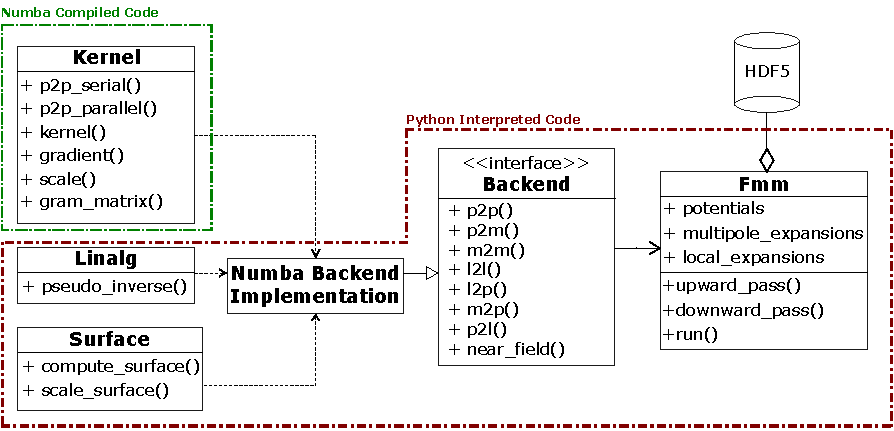
\includegraphics {figures/software.pdf}}
	\caption{Simplified UML model of all PyExaFMM components. Trees and operators are precomputed and stored in the HDF5 database. The `Fmm' object which acts as the user interface, all other components are modules consisting of methods on operating on arrays.}
	\label{fig:design}
\end{figure*}

\subsection{Parallelization Strategies for FMM operators}

Numba implements its threading layer in an agnostic way, compatible with OpenMP and Intel TBB backends, it also provides a generic cross-platform implementation. We choose the OpenMP backend, as the size of the tasks performed by FMM operators are approximately uniform. TBB implements scheduling optimizations, more suited to unbalanced workloads. BLAS routines called from within threads are multithreaded by default, leading to \textit{nested parallelism}. We avoid this by restricting these operations to run on a single thread.

PyExaFMM implements two parallelization strategies for FMM operators. For the P2M, L2P and P2P operators we allocate aligned arrays of the `sources' and `targets' for each target box being considered at a given level. For brevity, we overload the term `source' to refer local expansion points, and `target' to refer to multipole expansion points in the L2P and P2M operators, respectively. The kernel function, and its corresponding gradient function, are run in parallel over sources and targets, batched by their corresponding target box.

As we don't apriori know the size of the interaction lists for a given box, we have to allocate enough space at runtime to store the maximum possible number of sources and targets for each operator, and use \textit{index pointers} to lookup data for a given target box. Allocation cost is restricted by the constraint dictating the maximum number of particles per leaf box, and the order of the local and multipole expansions. For the P2P operator, cost is also restricted by the 2:1 balance condition, which limits the maximum size of the $U$ list to 60 in 3D. This strategy is optimized for cache re-use due to the aligned arrays.

For the M2L and M2P operators, the maximum size of the $V$ and $W$ lists for all boxes at a given level makes the above strategy expensive in terms of memory. In 3D, after imposing a 2:1 balance condition, a given target box has up to 189 source boxes in its $V$ list, and 148 in its $W$ list. For example, allocating an array to store the coordinates for source particles in double precision for boxes in the $W$ list of a uniform tree with 5 levels, hence 32768 target leaf boxes, with at most 150 particles per leaf box, requires $\sim 17$GB. Again, we overload the term `source' to refer to multipole expansion points in both operators, and `target' to refer to local expansion points the M2L operator. Instead, we perform a parallel loop over all target boxes at a given level. We don't optimize for CPU cache re-use as we look up data from an un-aligned global array.

The maximum size of the $X$ list for a given box is 19 in 3D, we observe empirically that this is too small to be impacted by the first strategy. Each thread, computing the S2L operation over a target box's $X$ list, contains relatively little computation. Therefore, it is computed in a similar way to the M2L and M2P operators.

Our implementation requires the computation of transfer vectors for each source box in a $V$ list within the M2L operator. Therefore, we needed to develop a `hash' function for transfer vectors, to look up the corresponding components of the compressed M2L operator (\ref{eq:compressed_m2l}). Numba offers an implementation of Python's built-in hash function, however it is not optimized, as it falls out of Numba's numerical remit. This is an example of where naive usage of native Python functions or objects can impact performance, despite being supported by Numba. We resolve this by computing a checksum for transfer vectors by uniquely mapping its components to the positive real integers, and concatenating them. This is optimized by Numba as we use only simple bit shifts and arithmetic operations.

\section{Benchmarks}

Benchmarks are taken on an Intel i7-9750H mobile workstation, running Ubuntu 20.04.2, GCC 9.3.0 and OpenMP 4.5. Timings are repeated 5 times for statistics, and standard deviation is used to describe error, and is reported to one significant figure.

Numba compilation makes many of PyExaFMM's functions competitive with ExaFMM-T's C++ implementation. Our implementation of (\ref{eq:laplace_kernel}) evaluates interactions between 100,000 sources and targets in $4.7 \pm 0.3$ s compared to $2.00 \pm 0.01$ s with ExaFMM-T. For a problem with 1,000,000 randomly distributed particles, and a constraint of at most 150 particles per leaf box, and depth 5, tree building and balancing takes $2.75 \pm 0.04$ s compared to $0.64 \pm 0.01$ s in ExaFMM-T. Operator pre-computation times depend on the expansion order of the multipole and local expansions, $p$, as the depth of the tree and compression rank $k$. It is fast enough not to significantly impact on workflow. For the above problem with $p=6$ expansions and $k=100$, it takes $5.01 \pm 0.2$ s to pre-compute all operators, for $k=152$ (full rank), it takes $8.00 \pm 0.3$ s.

Experiments in table (\ref{tab:performance}) measuring the accuracy, peak memory consumption, and runtimes of the two softwares are tested for two source and target particle distributions: randomly in a cubic unit box, and randomly on the surface of a sphere with unit radius. We test with 1,000,000 source and target particles, and a constraint of 150 particles per leaf box.

We observe that our implementation is bound by the M2L operator. Table (\ref{tab:performance}) shows how runtimes increase as a function of M2L compression rank $k$ for both particle distributions, and figure (\ref{fig:operator_runtimes}) shows how the M2L operator increasingly dominates PyExaFMM's runtime as a function of $k$. The M2L operator depends on loads from global memory, and is not cache-optimized due to the large memory requirements of doing so. We see that although compression significantly reduces runtimes, it does so at the expense of relative error. Importantly, from figure (\ref{fig:operator_runtimes}a) and (\ref{fig:operator_runtimes}b), where we test both softwares with the $p=6$ expansions and set $k=10$, we see that the FMM operators take similar proportions of total runtime, and from table (\ref{tab:performance}) we see that PyExaFMM remains $\mathcal{O}(10)$ slower. This implies that PyExaFMM applies an approximately constant overhead for a computing solutions at a given expansion order $p$ regardless of compression. The minimal design of PyExaFMM's interface, with most computation and memory management taking place within Numba compiled functions, implies that this overhead is attributable to the performance disadvantage of Python and Numba in comparison to C++.

% Smaller figure
\begin{figure}
	\centerline{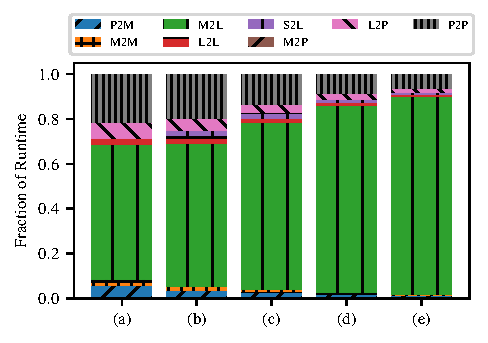
\includegraphics {figures/operator_runtimes.pdf}}
	\caption{Fractional runtimes broken down by operator for (a) ExaFMM-T $p=6$ (b) PyExaFMM $p=6$, $k=10$ (c) PyExaFMM $p=6$, $k=50$ (d) PyExaFMM $p=6$, $k=100$ (e) PyExaFMM $p=6$, $k=188$ (full rank)}
	\label{fig:operator_runtimes}
\end{figure}

\begin{table*}
	\centering
	\caption{PyExaFMM (Py) vs ExaFMM-T (Ex-T). Number of particles $N=$1,000,000 leading to $M$ leaves in a given geometry. $k$ is the compression rank for PyExaFMM. Charge densities are chosen in the interval $[0, 1)$. Runtimes exclude precomputations. Memory usage and relative error reported to 3 s.f.}
	\begin{tabular*}{0.934\textwidth}{|*{10}{c|}}
		\hline
		& & &   & \multicolumn{2}{c|}{Runtime} & \multicolumn{2}{c|}{Peak Memory} & \multicolumn{2}{c|}{Relative Error}\\
		\hline
		$p$ & $M$ &$k$ &  Geometry   &   Py  &  Ex-T &    Py  &  Ex-T  &   Py  &  Ex-T\\
		\hline
		6 & 17,017 & 10 &   Sphere  &  $10.7 \pm 0.3$ s & $0.92 \pm 0.03$ s  &  2.64 GB  &  1.96 GB  & 4.64e-4 & 3.82e-7 \\
		 & 32,768 &    &   Random  &  $17.5 \pm 0.3$ s &  $1.10 \pm 0.03$ s &  4.66 GB  &  2.04 GB  & 1.46e-4 &  3.31e-7\\
		 & & 100   &   Sphere  &  $13.6 \pm 0.3$ s &   &  2.66 GB  &   & 4.58e-7 &  \\
		 & &    &   Random  &  $36.7 \pm 0.4$ s &  &  4.68 GB  &  & 3.96e-7 & \\
		 & & Full Rank  &   Sphere  &  $15.8 \pm 0.1$ s &   &  2.70 GB  &  & 4.61e-7 & \\
		 & & (152) &   Random  &  $50.5 \pm 0.7$ s &   &  4.72 GB  &  & 3.94e-7 & \\
		\hline
	\end{tabular*}
	\label{tab:performance}
 \end{table*}

\section{CONCLUSION}

In this paper we've shown how to use Numba to create a performant application for an algorithm with a complex data structure. We've shown how Numba can constrain software design, and that developers must be careful in designing methods and data structures in order to experience a performance benefit. Furthermore, performance debugging for more complex applications may require more knowledge than novice users can be expected to have, for example in optimizing the performance of multithreaded applications. Therefore, despite being trivial to `drop-in' to an existing application, Numba can be seen to have its own learning curve for achieving performance.

Furthermore, Numba is not able to optimize applications with significant array manipulations or allocations. We see this reflected in PyExaFMM's poor runtime performance in comparison to ExaFMM-T. Despite this, we conclude that Numba is a remarkable tool. With a great deal of functionality, allowing one to develop fast, heterogenous, cross-platform numerical applications, using only Python. Performance for PyExaFMM is still good, and it offers a platform for experimentation and prototyping, despite not being suitable for HPC.

\section{ACKNOWLEDGMENT}

SK is supported by EPSRC Studentship 2417009.

% \vspace{50pt}
\bibliography{pyexafmm}

\bibliographystyle{ieeetr}

\begin{IEEEbiography}{Srinath Kailasa}{\,}is a PhD student in Mathematics at University College London. Contact him at srinath.kailasa.18@ucl.ac.uk.
\end{IEEEbiography}

\begin{IEEEbiography}{Tingyu Wang}{\,}is a PhD student in Mechanical Engineering at the George Washington University. Contact him at twang66@email.gwu.edu.
\end{IEEEbiography}

\begin{IEEEbiography}{Lorena. A. Barba}{\,}is a Professor of Mechanical and Aerospace Engineering at the George Washington University.  Contact her at labarba@email.gwu.edu.
\end{IEEEbiography}

\begin{IEEEbiography}{Timo Betcke}{\,}is Professor of Computational Mathematics at University College London. Contact him at t.betcke@ucl.ac.uk.
\end{IEEEbiography}
\end{document}

